% =============================================================================
% PART B - MODULE 14: ADMINISTRATOR RBAC & USER MANAGEMENT (M14.01 - M14.08)
% In Charge: Nguyen Tien Thuan (CE181024)
% =============================================================================

\newpage
\subsection{Module 14: Administrator System, RBAC \& User Management}

The Administrator System, RBAC, and User Management module empowers system governors with a centralized management console (\textit{Admin Portal}). From this single pane of glass, administrators can monitor cross-platform operational metrics, configure fine-grained \textbf{Role-Based Access Control (RBAC)} down to specific API endpoints (\textit{HTTP Method + Path}), and oversee user account lifecycles along with their specialized multi-profile identities.

% -----------------------------------------------------------------------------
\subsubsection{M14.01 -- Administrator Central Operations Dashboard (\texttt{/admin})}

\begin{itemize}[leftmargin=1.5em,itemsep=2pt]
  \item \textbf{Screen Name \& Route Path:} Administrator Dashboard -- \texttt{/admin}.
  \item \textbf{Target Actor:} Administrator.
  \item \textbf{Preconditions:} Authenticated user holds the \texttt{ADMIN} role in good standing.
\end{itemize}

\begin{figure}[H]
  \centering
  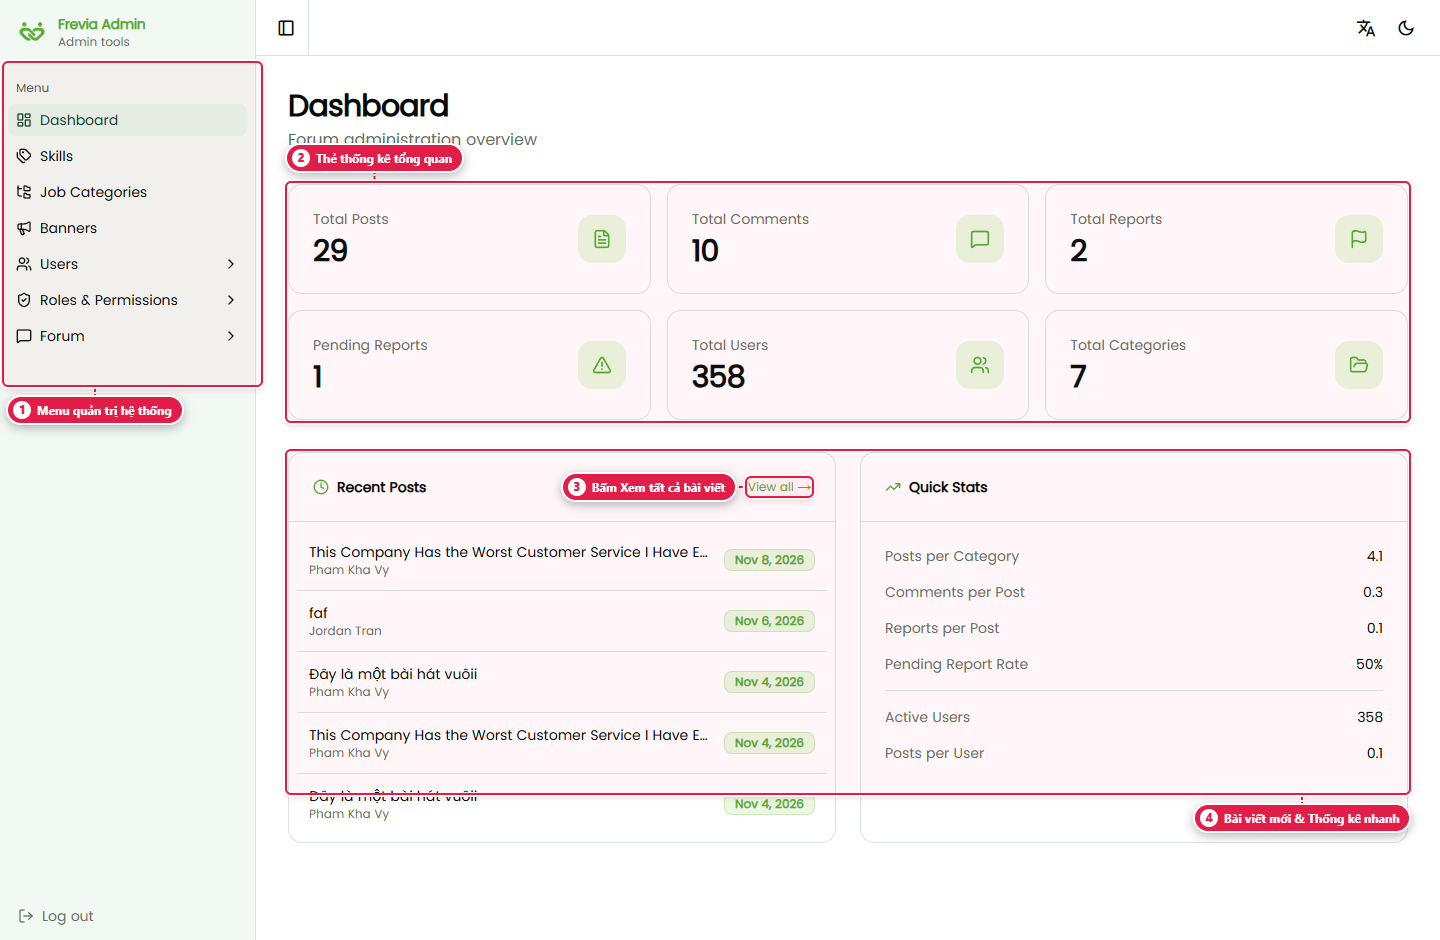
\includegraphics[width=0.90\textwidth]{images/admin/m14_01_admin_dashboard.png}
  \caption{Central Administrator Dashboard and operational KPI metrics at \texttt{/admin}}
\end{figure}

\paragraph{Step-by-Step User Instructions:}
\begin{enumerate}[leftmargin=1.8em,itemsep=3pt]
  \item \rbadge{1} \textbf{Navigate via Admin Sidebar (\textit{Navigation menu}):} Utilize the left sidebar to navigate across management subsystems: \textit{Dashboard}, \textit{Skills}, \textit{Job Categories}, \textit{Banners}, the \textit{Users} group (\textit{User Management}, \textit{Identity Verification}, \textit{Profile Reviews}), the \textit{Roles \& Permissions} group (\textit{Roles}, \textit{Permissions}, \textit{Assign Role}), and the \textit{Forum} group.
  \item \rbadge{2} \textbf{Review Platform Operational KPIs (\textit{Overview stat cards}):} Monitor 6 real-time operational indicators: \textit{Total Posts}, \textit{Total Comments}, \textit{Total Reports}, \textit{Pending Reports}, \textit{Total Users}, and \textit{Total Categories}.
  \item \rbadge{3} \textbf{Navigate to Posts Catalog (\textit{View all $\rightarrow$}):} In the \textit{Recent Posts} panel, inspect recent publications, authors, and timestamps; click \textbf{View all $\rightarrow$} to access the comprehensive moderation table at \texttt{/admin/posts}.
  \item \rbadge{4} \textbf{Inspect Analytics Breakdown (\textit{Quick stats}):} Examine platform ratios on the right panel, including \textit{Posts per Category}, \textit{Comments per Post}, \textit{Pending Report Rate}, and current \textit{Active Users}.
\end{enumerate}

\paragraph{Expected Output \& Exception Handling:}
\begin{itemize}[leftmargin=1.5em,itemsep=2pt]
  \item \textbf{Success Scenario:} All analytics synchronize dynamically with the underlying database.
  \item \textbf{Exception Scenarios:} If an unprivileged user navigates to \texttt{/admin}, the authorization guard intercepts the request and redirects to \texttt{/access-denied?requiredRole=admin}.
\end{itemize}

% -----------------------------------------------------------------------------
\newpage
\subsubsection{M14.02 -- Administrator Profile, Identity \& System Privileges (\texttt{/admin/users/1})}

\begin{itemize}[leftmargin=1.5em,itemsep=2pt]
  \item \textbf{Screen Name \& Route Path:} Administrator Profile \& Privileges View -- \texttt{/admin/users/1}.
  \item \textbf{Target Actor:} Administrator.
  \item \textbf{Preconditions:} Administrator is signed in and authorized.
\end{itemize}

\begin{figure}[H]
  \centering
  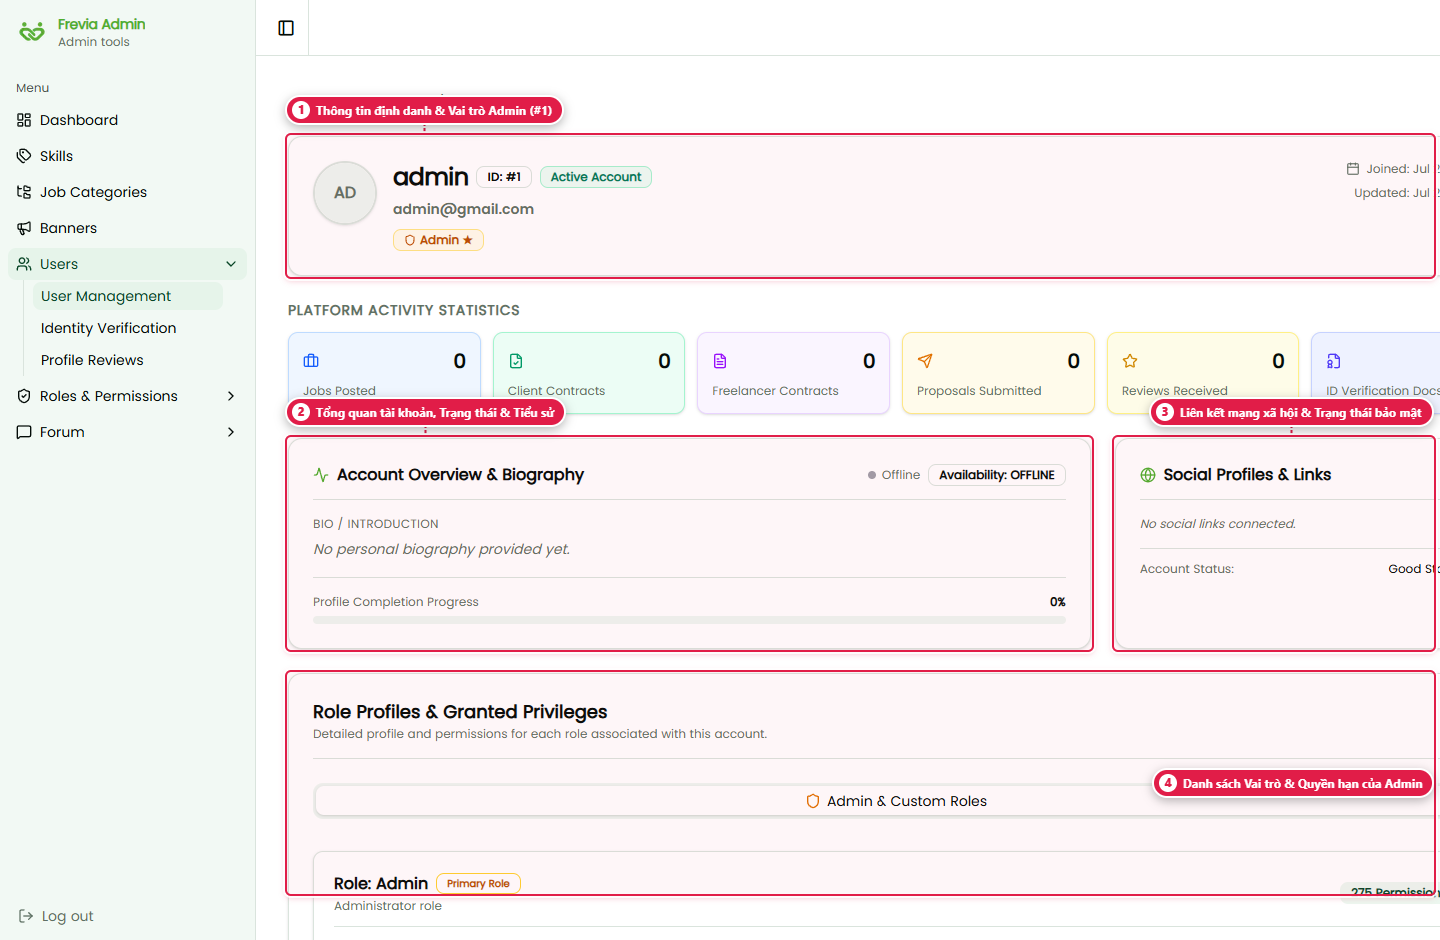
\includegraphics[width=0.90\textwidth]{images/admin/m14_02_admin_profile.png}
  \caption{Administrator profile identity, standing, and granted privileges at \texttt{/admin/users/1}}
\end{figure}

\paragraph{Step-by-Step User Instructions:}
\begin{enumerate}[leftmargin=1.8em,itemsep=3pt]
  \item \rbadge{1} \textbf{Review Core Identity Information (\#1):} Inspect the primary identity card displaying Avatar, Display Name (\texttt{admin}), User ID (\texttt{ID: \#1}), account standing badge (\textbf{Active Account}), Email (\texttt{admin@gmail.com}), and the \textbf{Admin $\star$} role badge.
  \item \rbadge{2} \textbf{Inspect Account Standing \& Bio (\textit{Overview \& Bio}):} Review online connectivity status, biographical summary, and profile completeness indicator.
  \item \rbadge{3} \textbf{Review Social Links \& Security Standing (\textit{Social Profiles}):} Verify linked social identity bindings and account trust scores.
  \item \rbadge{4} \textbf{Audit Assigned System Privileges (\textit{Role Profiles \& Privileges}):} Click the \textbf{Admin \& Custom Roles} tab to review the complete list of all 275 assigned API permissions. Administrator details can be updated via the \textit{Edit user} dialog on the user management page (\texttt{/admin/users}).
\end{enumerate}

\paragraph{Expected Output \& Exception Handling:}
\begin{itemize}[leftmargin=1.5em,itemsep=2pt]
  \item \textbf{Success Scenario:} Detailed administrative authority and system credentials are transparently presented for auditability.
\end{itemize}

% -----------------------------------------------------------------------------
\newpage
\subsubsection{M14.03 -- System Roles \& Custom Roles Management (UC-06.01 to UC-06.05)}

\begin{itemize}[leftmargin=1.5em,itemsep=2pt]
  \item \textbf{Screen Name \& Route Path:} Roles Management Console -- \texttt{/admin/roles}.
  \item \textbf{Target Actor:} Administrator.
  \item \textbf{Preconditions:} Access to \texttt{ADMIN\_ROLES} module permissions.
\end{itemize}

\begin{figure}[H]
  \centering
  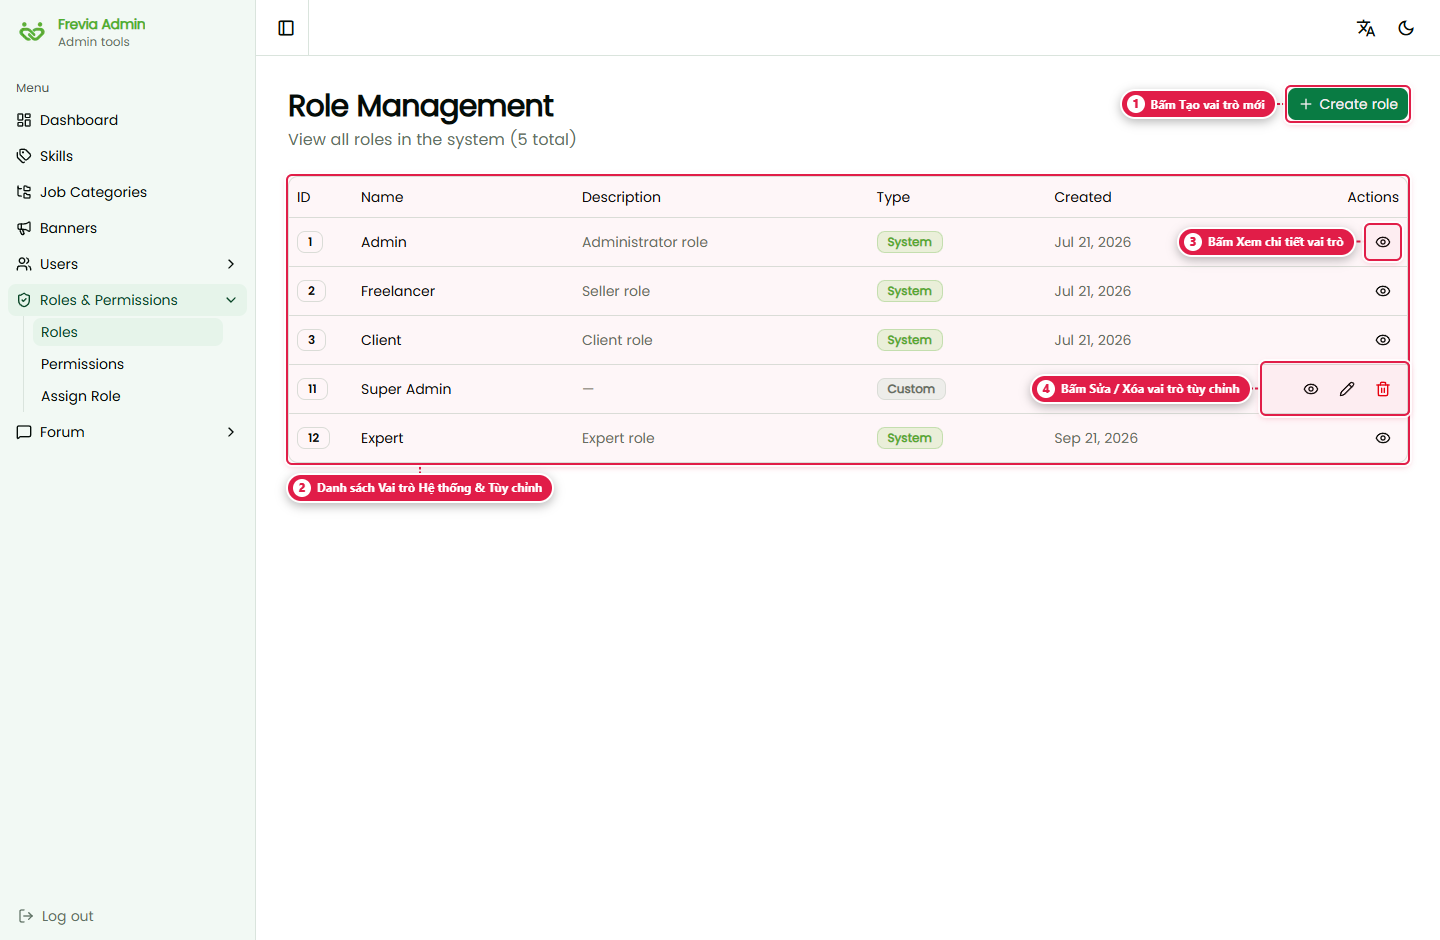
\includegraphics[width=0.90\textwidth]{images/admin/m14_03_admin_roles.png}
  \caption{System and Custom Roles management console at \texttt{/admin/roles}}
\end{figure}

\paragraph{Step-by-Step User Instructions:}
\begin{enumerate}[leftmargin=1.8em,itemsep=3pt]
  \item In the Admin sidebar, navigate to \textbf{Roles \& Permissions} $\rightarrow$ \textbf{Roles}.
  \item \rbadge{1} \textbf{Search Roles (\textit{Search input}):} Filter records by role name (e.g., \texttt{ADMIN}, \texttt{FREELANCER}, \texttt{CLIENT}, \texttt{EXPERT}, \texttt{MODERATOR}).
  \item \rbadge{2} \textbf{Create New Role (\textit{+ Create Role}):} Click \textbf{+ Create Role} to launch a dialog where custom roles (e.g., \textit{Moderator}, \textit{Auditor}) can be defined with a Name and Description.
  \item \rbadge{3} \textbf{Inspect Roles Table (\textit{Roles Table}):} View listed roles with their \textit{ID}, \textit{Name}, \textit{Description}, \textit{Type} (distinguishing unalterable core \textbf{System Roles} from user-created \textbf{Custom Roles}), and creation timestamps.
  \item \rbadge{4} \textbf{Perform Role Actions (\textit{Actions column}):}
    \begin{itemize}
      \item Click the shield key icon (\textbf{Shield icon}) to open the permission assignment matrix for that role.
      \item Click the pencil icon (\textbf{Pencil icon}) to update custom role metadata.
      \item Click the red trash icon (\textbf{Trash icon}) to delete custom roles. Core system roles are locked to prevent accidental deletion.
    \end{itemize}
\end{enumerate}

\paragraph{Expected Output \& Exception Handling:}
\begin{itemize}[leftmargin=1.5em,itemsep=2pt]
  \item \textbf{Success Scenario:} New roles are immediately available across the user management and permission assignment interfaces.
  \item \textbf{Exception Scenarios:} The backend enforces a uniqueness constraint on role names and rejects attempts to delete default system roles.
\end{itemize}

% -----------------------------------------------------------------------------
\newpage
\subsubsection{M14.04 -- Dynamic Role-Permission Assignment Matrix (UC-06.06)}

\begin{itemize}[leftmargin=1.5em,itemsep=2pt]
  \item \textbf{Screen Name \& Route Path:} Role Permission Assignment Matrix -- \texttt{/admin/assign-role}.
  \item \textbf{Target Actor:} Administrator.
  \item \textbf{Preconditions:} Administrator has permissions to assign RBAC rights.
\end{itemize}

\begin{figure}[H]
  \centering
  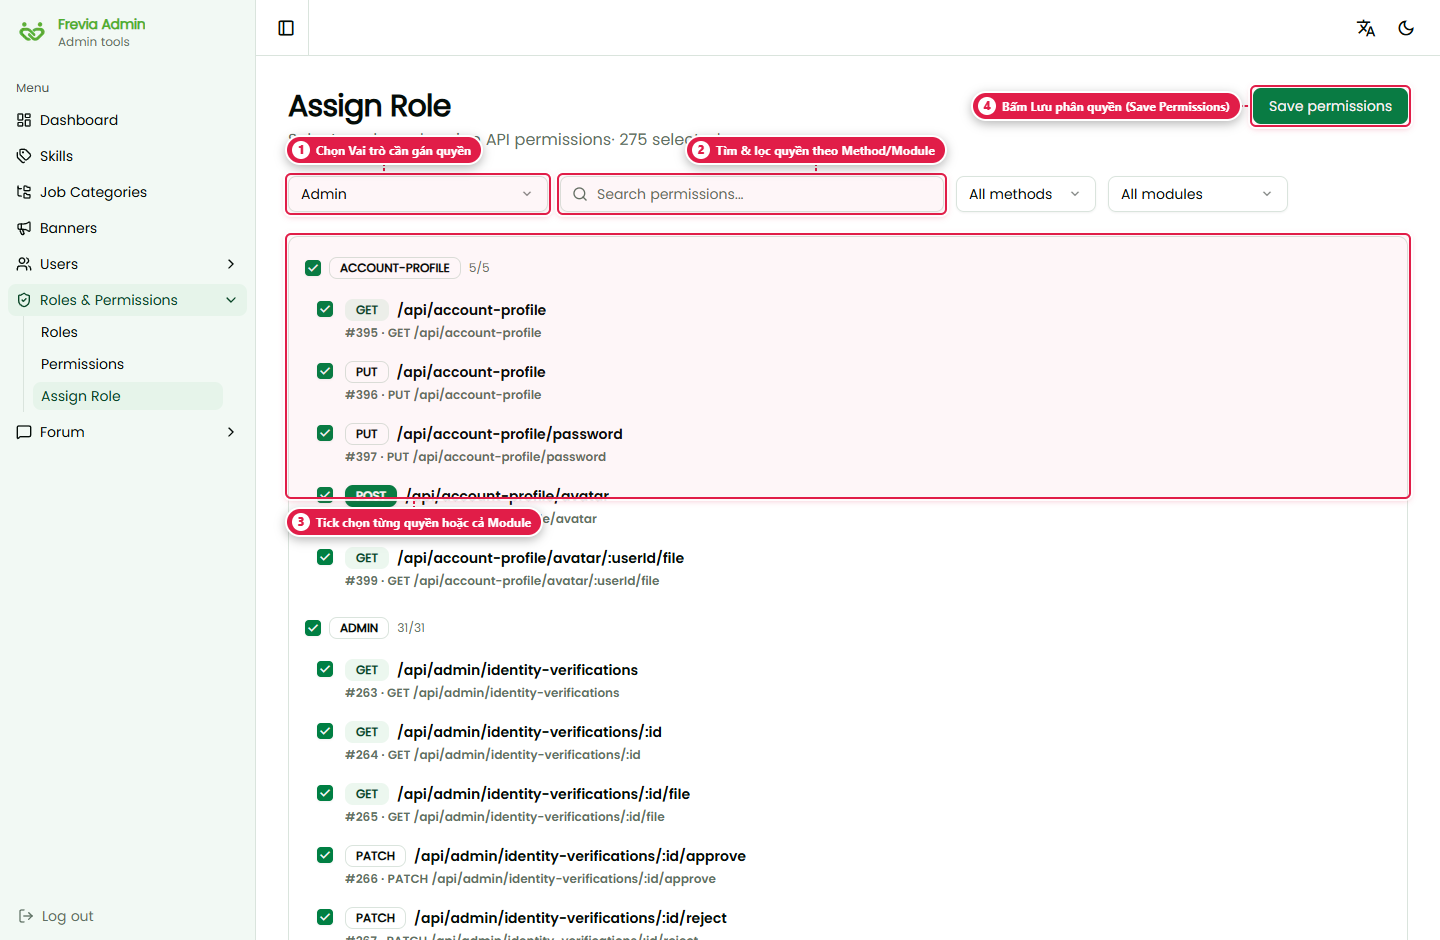
\includegraphics[width=0.90\textwidth]{images/admin/m14_04_role_permissions_matrix.png}
  \caption{Dynamic RBAC role-permission matrix configuration at \texttt{/admin/assign-role}}
\end{figure}

\paragraph{Step-by-Step User Instructions:}
\begin{enumerate}[leftmargin=1.8em,itemsep=3pt]
  \item In the Admin sidebar, navigate to \textbf{Roles \& Permissions} $\rightarrow$ \textbf{Assign Role}.
  \item \rbadge{1} \textbf{Select Target Role (\textit{Select Role dropdown}):} Choose the role to configure (e.g., \texttt{ADMIN}, \texttt{FREELANCER}, \texttt{CLIENT}, \texttt{EXPERT}).
  \item \rbadge{2} \textbf{Persist Matrix Changes (\textit{Save Changes}):} After toggling permissions, click the green \textbf{Save Changes} button to commit updates to the database.
  \item \rbadge{3} \textbf{Toggle Permissions by Module (\textit{Permission Matrix}):} Scroll through permission groups organized by domain modules (\textit{AUTH}, \textit{USERS}, \textit{ROLES}, \textit{SKILLS}, \textit{JOBS}, \textit{PROPOSALS}, \textit{CONTRACTS}, \textit{PAYMENTS}, \textit{REVIEWS}). Toggle switches to grant or revoke specific API endpoints.
  \item \rbadge{4} \textbf{Batch Module Toggles (\textit{Select All / Deselect All}):} Click module-level headers to toggle all contained permissions in a single action.
\end{enumerate}

\paragraph{Expected Output \& Exception Handling:}
\begin{itemize}[leftmargin=1.5em,itemsep=2pt]
  \item \textbf{Success Scenario:} The server updates the \texttt{RolePermission} junction table. NestJS guards evaluate these updated permissions on subsequent requests without requiring server reboots.
\end{itemize}

% -----------------------------------------------------------------------------
\newpage
\subsubsection{M14.05 -- System API Permission Catalog \& Multi-Criteria Filtering (UC-15.01 to UC-15.04)}

\begin{itemize}[leftmargin=1.5em,itemsep=2pt]
  \item \textbf{Screen Name \& Route Path:} Permissions Catalog -- \texttt{/admin/permissions}.
  \item \textbf{Target Actor:} Administrator.
  \item \textbf{Preconditions:} Access to \texttt{ADMIN\_PERMISSIONS} module.
\end{itemize}

\begin{figure}[H]
  \centering
  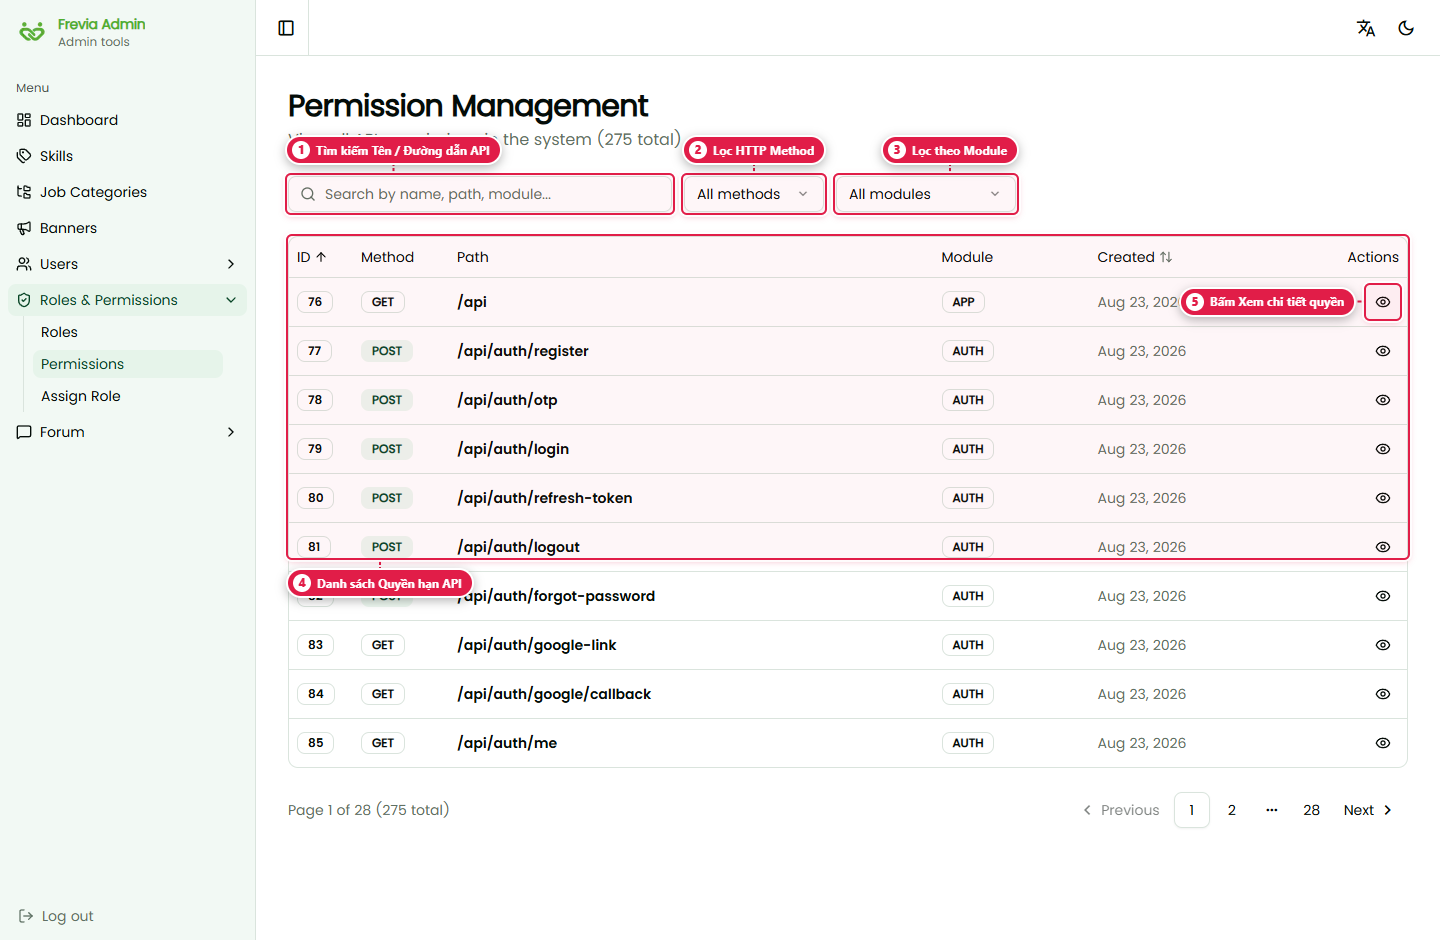
\includegraphics[width=0.90\textwidth]{images/admin/m14_05_admin_permissions.png}
  \caption{System API Permission catalog with method and module filters at \texttt{/admin/permissions}}
\end{figure}

\paragraph{Step-by-Step User Instructions:}
\begin{enumerate}[leftmargin=1.8em,itemsep=3pt]
  \item In the Admin sidebar, click \textbf{Roles \& Permissions} $\rightarrow$ \textbf{Permissions}.
  \item \rbadge{1} \textbf{Search Permissions by Name or Path (\textit{Search box}):} Input keywords matching permission names (e.g., \texttt{CREATE\_JOB}), paths (e.g., \texttt{/jobs}), or descriptions.
  \item \rbadge{2} \textbf{Filter by HTTP Method (\textit{Method filter}):} Select an HTTP verb from the dropdown (\textit{ALL}, \textit{GET}, \textit{POST}, \textit{PUT}, \textit{PATCH}, \textit{DELETE}) to isolate specific operations.
  \item \rbadge{3} \textbf{Filter by Domain Module (\textit{Module filter}):} Select a functional module (e.g., \textit{AUTH}, \textit{USERS}, \textit{JOBS}, \textit{CONTRACTS}, \textit{PAYMENT}) to view its endpoints.
  \item \rbadge{4} \textbf{Inspect Permissions Table (\textit{Permissions table}):} View permission records with \textit{ID}, \textit{Name}, color-coded \textit{Method} badges (Blue for GET, Green for POST, Amber for PUT, Red for DELETE), \textit{Path}, and \textit{Module}.
\end{enumerate}

\paragraph{Expected Output \& Exception Handling:}
\begin{itemize}[leftmargin=1.5em,itemsep=2pt]
  \item \textbf{Success Scenario:} Instantaneous client-side and server-side filtering across the entire catalog of 275 system endpoints.
\end{itemize}

% -----------------------------------------------------------------------------
\newpage
\subsubsection{M14.06 -- User Directory Administration \& Direct Account Provisioning (UC-07.01 to UC-07.03)}

\begin{itemize}[leftmargin=1.5em,itemsep=2pt]
  \item \textbf{Screen Name \& Route Path:} User Management Console -- \texttt{/admin/users}.
  \item \textbf{Target Actor:} Administrator.
  \item \textbf{Preconditions:} Access to \texttt{ADMIN\_USERS} module.
\end{itemize}

\begin{figure}[H]
  \centering
  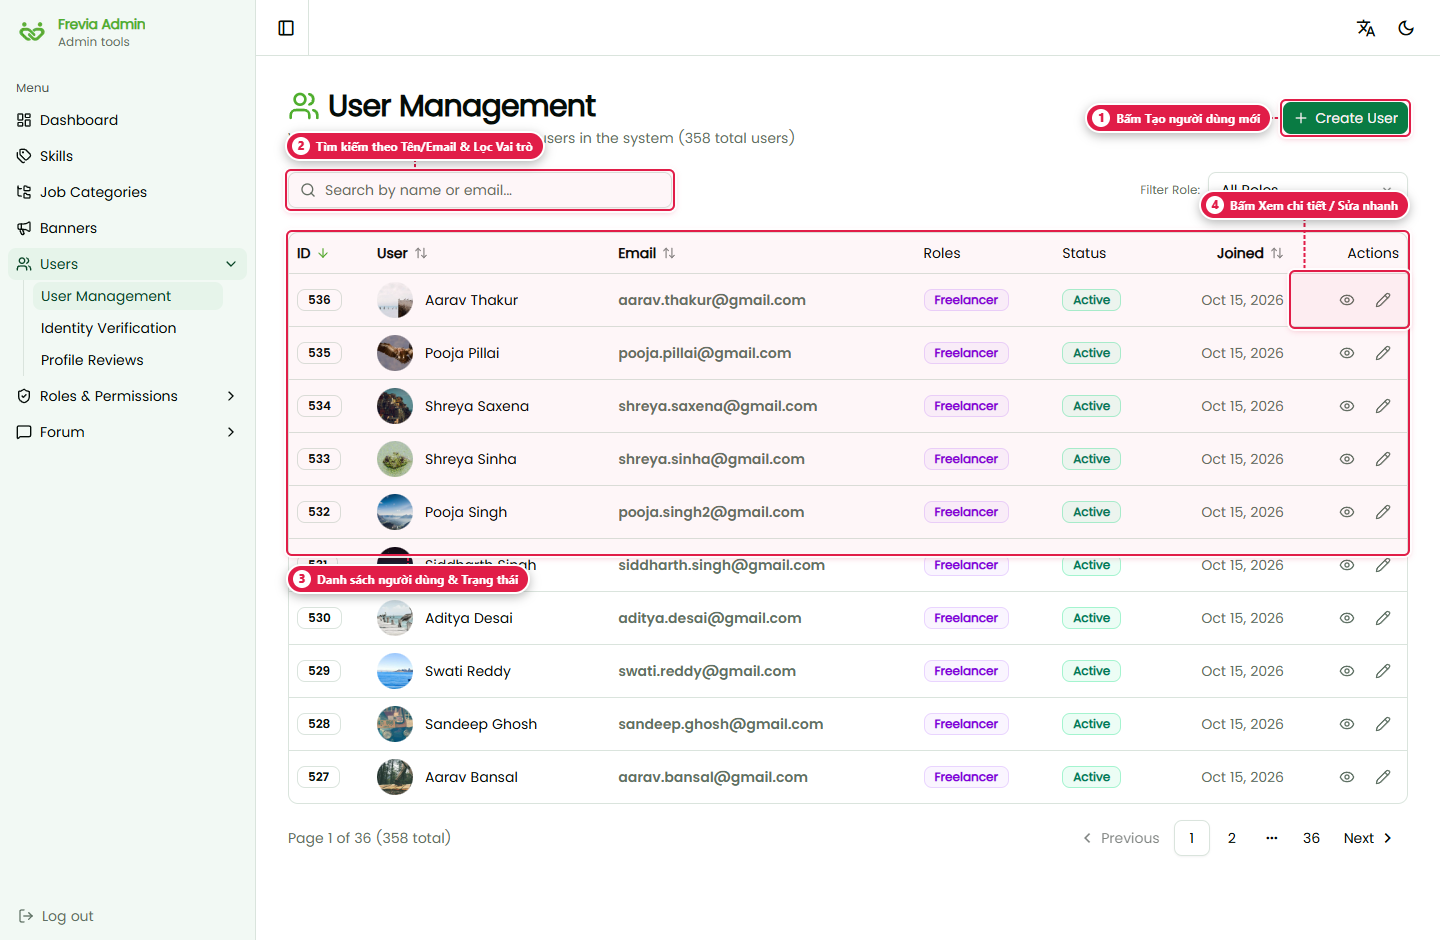
\includegraphics[width=0.90\textwidth]{images/admin/m14_06_admin_users_list_create.png}
  \caption{User directory table and account provisioning interface at \texttt{/admin/users}}
\end{figure}

\paragraph{Step-by-Step User Instructions:}
\begin{enumerate}[leftmargin=1.8em,itemsep=3pt]
  \item In the Admin sidebar, click \textbf{Users} $\rightarrow$ \textbf{User Management}.
  \item \rbadge{1} \textbf{Search Users by Name or Email (\textit{Search input}):} Type a query to search across user records in real time.
  \item \rbadge{2} \textbf{Filter Accounts by Standing (\textit{Status filter}):} Select \textit{All}, \textit{Active}, or \textit{Banned} from the status dropdown.
  \item \rbadge{3} \textbf{Direct Account Provisioning (\textit{+ Create User}):} Click \textbf{+ Create User} to open the modal dialog, input Full Name, Email, Password, and assign initial roles.
  \item \rbadge{4} \textbf{Inspect User Table \& Row Actions (\textit{Users Table \& Actions}):} Review user attributes (\textit{ID}, \textit{Name}, \textit{Email}, \textit{Status}, \textit{Roles}, \textit{Created}). On each row:
    \begin{itemize}
      \item Click the eye icon (\textbf{Eye icon}) to open the user's multi-profile details view (\texttt{/admin/users/[id]}).
      \item Click the pencil icon (\textbf{Pencil icon}) to open the \textit{Edit user} modal dialog.
    \end{itemize}
\end{enumerate}

\paragraph{Expected Output \& Exception Handling:}
\begin{itemize}[leftmargin=1.5em,itemsep=2pt]
  \item \textbf{Success Scenario:} Administrators maintain full directory oversight and can provision verified staff accounts directly.
\end{itemize}

% -----------------------------------------------------------------------------
\newpage
\subsubsection{M14.07 -- User Account Status Management \& Suspension/Reactivation (UC-07.04 to UC-07.05)}

\begin{itemize}[leftmargin=1.5em,itemsep=2pt]
  \item \textbf{Screen Name \& Route Path:} Edit User Dialog -- \texttt{/admin/users}.
  \item \textbf{Target Actor:} Administrator.
  \item \textbf{Preconditions:} Target user account exists in the system.
\end{itemize}

\begin{figure}[H]
  \centering
  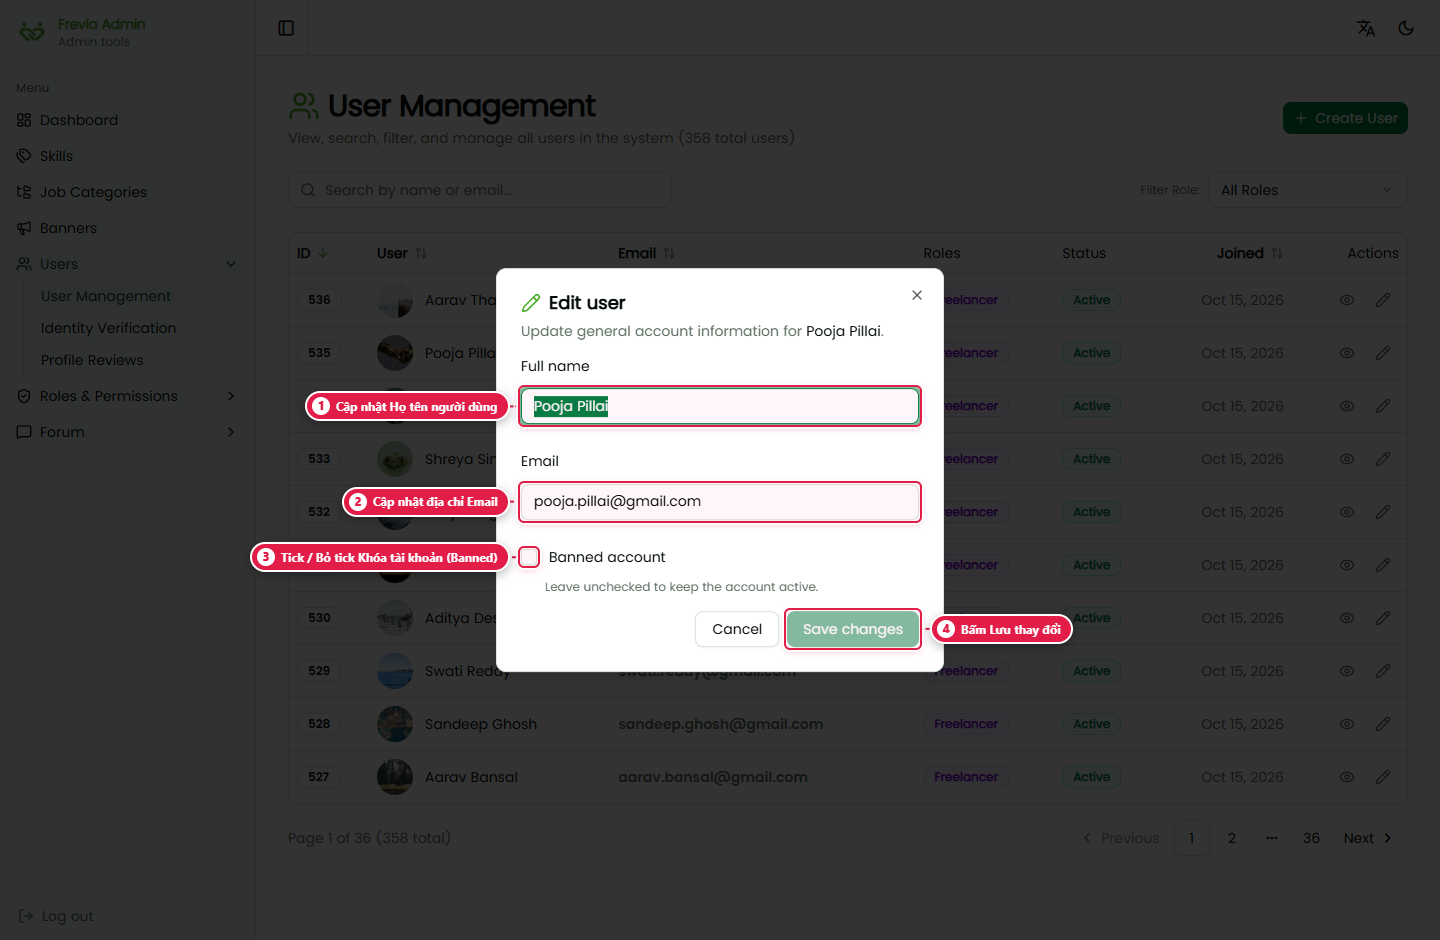
\includegraphics[width=0.90\textwidth]{images/admin/m14_07_admin_user_ban_unban.png}
  \caption{Edit User modal dialog featuring the Banned account toggle at \texttt{/admin/users}}
\end{figure}

\paragraph{Step-by-Step User Instructions:}
\begin{enumerate}[leftmargin=1.8em,itemsep=3pt]
  \item \rbadge{1} \textbf{Open Edit User Dialog:} Click the pencil icon on any user row in \texttt{/admin/users}. The modal header displays \textit{"Edit User -- Update user profile and manage account status"}.
  \item \rbadge{2} \textbf{Edit Full Name (\textit{Full Name field}):} Modify the user's name if required.
  \item \rbadge{3} \textbf{Edit Email Address (\textit{Email field}):} Update the primary email address if necessary.
  \item \rbadge{4} \textbf{Toggle Account Suspension (\textit{Banned account checkbox}):}
    \begin{itemize}
      \item \textbf{Suspend Account:} Check \textit{"Banned account -- Check to ban this user from accessing the system"}.
      \item \textbf{Reactivate Account:} Uncheck the box to restore the user account to \textbf{Active} status.
      \item Click \textbf{Save changes} to apply the update.
    \end{itemize}
\end{enumerate}

\paragraph{Expected Output \& Exception Handling:}
\begin{itemize}[leftmargin=1.5em,itemsep=2pt]
  \item \textbf{Success Scenario:} Setting \texttt{isBanned = true} immediately invalidates all active sessions for that user. Subsequent sign-in attempts by that account will be blocked with an account suspension notification.
\end{itemize}

% -----------------------------------------------------------------------------
\newpage
\subsubsection{M14.08 -- Comprehensive User Multi-Profile Management (UC-07.06 to UC-07.07)}

\begin{itemize}[leftmargin=1.5em,itemsep=2pt]
  \item \textbf{Screen Name \& Route Path:} Multi-Profile Inspection View -- \texttt{/admin/users/[id]}.
  \item \textbf{Target Actor:} Administrator.
  \item \textbf{Preconditions:} User holds multi-role profile records (e.g., User \#2 holding Client and Freelancer identities).
\end{itemize}

\begin{figure}[H]
  \centering
  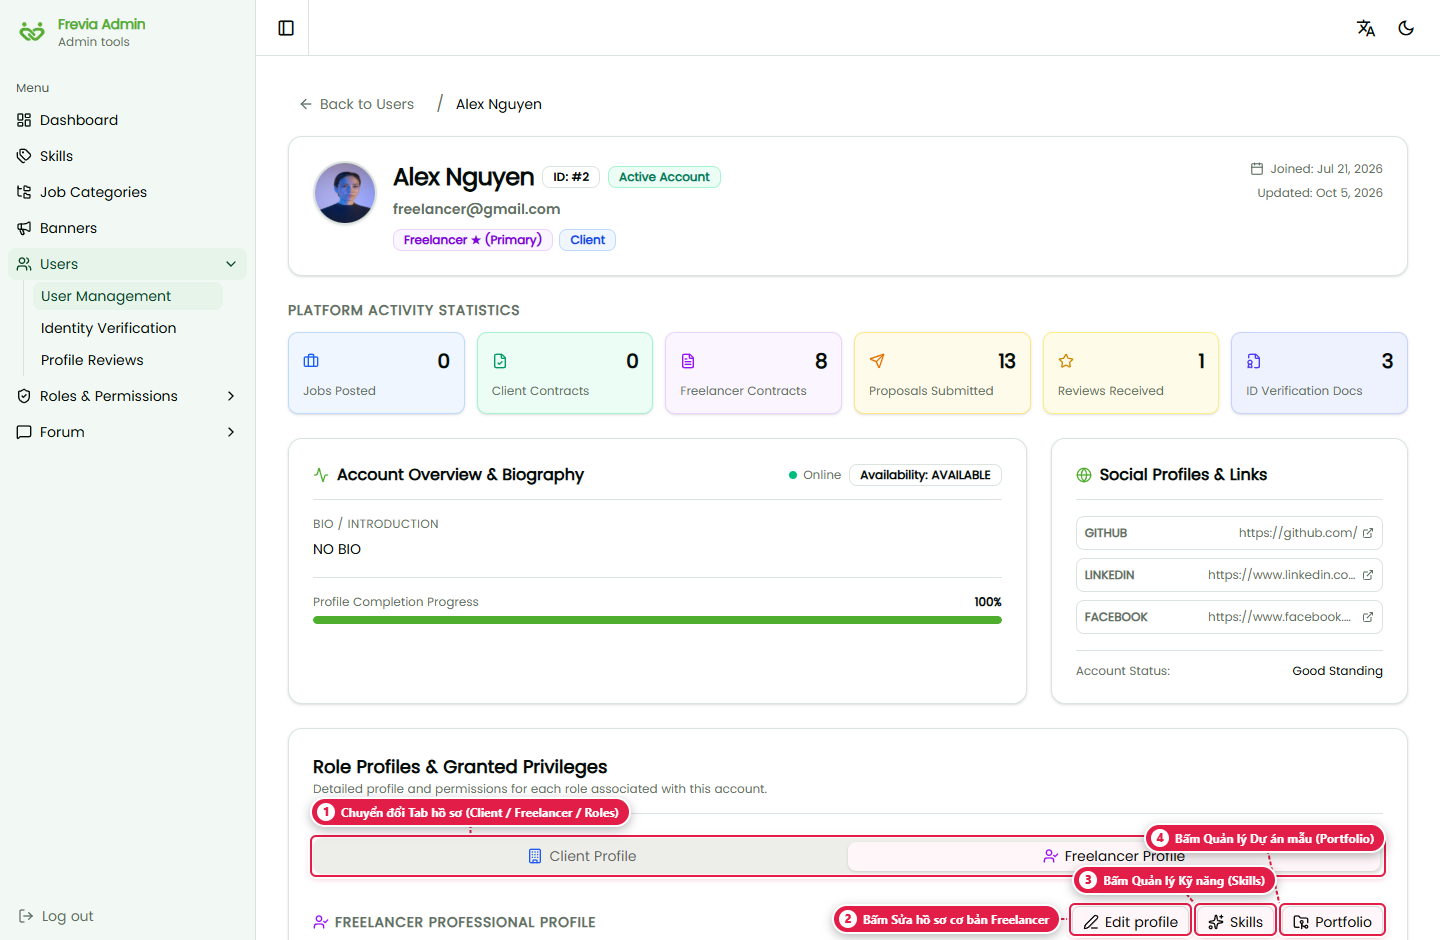
\includegraphics[width=0.90\textwidth]{images/admin/m14_08_admin_user_profile_tabs.png}
  \caption{Admin inspection view of dual Client and Freelancer profiles at \texttt{/admin/users/2}}
\end{figure}

\paragraph{Step-by-Step User Instructions:}
\begin{enumerate}[leftmargin=1.8em,itemsep=3pt]
  \item Navigate to \texttt{/admin/users/2} (or click the eye icon for that user in the directory).
  \item \rbadge{1} \textbf{Inspect Multi-Role Identity Badges:} Review the user header displaying Avatar, Display Name, Email, and active role badges (\textbf{Client}, \textbf{Freelancer}).
  \item \rbadge{2} \textbf{Switch Between Profile Tabs (\textit{Navigation tabs}):} Select from the available domain tabs: \textbf{Client Profile}, \textbf{Freelancer Profile}, \textbf{Skills \& Experience}, and \textbf{Portfolio}.
  \item \rbadge{3} \textbf{Inspect Client Profile Metrics (\textit{Client profile overview}):} Under \textit{Client Profile}, examine Company Name, Website, Payment Verification Status, Total Posted Jobs, and Total Spend.
  \item \rbadge{4} \textbf{Inspect Freelancer Profile Metrics (\textit{Freelancer profile overview}):} Under \textit{Freelancer Profile}, examine Professional Title, Hourly Rate, Completed Jobs, Total Earnings, and Bio.
\end{enumerate}

\paragraph{Expected Output \& Exception Handling:}
\begin{itemize}[leftmargin=1.5em,itemsep=2pt]
  \item \textbf{Success Scenario:} The administrator can seamlessly inspect and audit both sides of a dual-role user account without having to log in as that user.
\end{itemize}
